
\chapter{Methodology}

\matteo{We first need to explain what we are doing here. We gave lots of info about fuzzing, sanitizers etc. but we did not explain yet what we are doing and why.}

\matteo{Start this intro by saying these things, say that we want to see if there are overlooked bugs in common fuzzing benchmarks; we selected these two frameworks because they are among the most used and popular ones...; we looked for information that could hide overlooked bugs and we came up with fuzzing queues (OF) and old bugs (FB).}

\matteo{One interesting piece of narrative Daniele and I came up with is the following: finding bugs in OSS-Fuzz means highlighting machine-driven fuzz testing's mistakes (i.e. OSS-Fuzz is fully automated, finding overlooked bugs there means finding where machines fail, in that case). Finding bugs in FuzzBench, on the other hand, means finding bugs from older crashes (I mean, crashes from older version) that security researchers found but did not test on latest versions to see if they were still present, so humans are to blame in that case.}


\section{OSS-Fuzz}
\subsection{Selecting the projects} \label{selection}
At the moment of writing, the OSS-Fuzz campaign includes over 1000 projects that are actively fuzzed and tested, but it would obviously be impossible to rebuild and test all of them locally also due to the language heterogeneity of such projects.
\newline
For this reason, this work focused solely on projects using the C/C++ language.
\newline
Then, to further narrow down the analysis, I identified 5 different categories of projects using the number of sanitizers used by the developers, keeping ASan as the reference due to its popularity and efficiency.
\newline
Finally, I ordered each set by "highest number of bugs issued" using the OSS-Fuzz bug tracker and tested these lists top-down until I had 5 projects for each category that were building and fuzzing correctly.
\ \\ \newline \newline
First step in this process was to extract the list of all projects written in C/C++, and this was done by performing a preliminary analysis of the \textit{project.yaml} configuration file present inside each project's directory.
\newline
\begin{figure}[h]
\centering
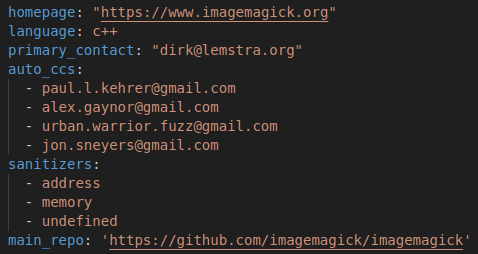
\includegraphics[scale=0.5]{foto/project_yaml.png}
\caption{Example of content from a project.yaml}
\label{fig:project_yaml}
\end{figure}
\ \\
To retrieve the language used by each project, I initially wrote a simple Python script taking as input the OSS-Fuzz "project" directory.
\newline
Then, the script retrieved the directory list of the argument provided and iteratively explored each project's directory looking for the aforementioned configuration file: assuming the file was found, it then opened the file and scanned each line looking for the "language: c" string, eventually saving the name of such projects in a list.
\newline \newline
This yielded a total of 524 projects out of 1277 written using C/C++.


\newpage
To perform the categorization of the projects depending on the number of sanitizers used, I extended the previous script to also look for the strings "address", "memory" and "undefined", shown on image \ref{fig:project_yaml}.
\newline
The assignment uses a binary logic on decimal values, starting each project from 0 and giving each sanitizer a different value (1, 10, 100), so that by summing them I could easily understand which sanitizers were found in its configuration file.
\newline \newline
Out of the previous 524 projects, the results were as follows: 238 used all sanitizers, 22 used ASan and MSan, 62 used ASan and UBSan, 46 used only ASan and 156 did not use any sanitizers.
\ \\ \newline \newline
The next step was retrieving the number of discovered bugs of each project, and this required a thorough analysis of the "OSS-Fuzz Issue Tracker" website. \cite{ossfuzz_bugtracker}
\newline
\begin{figure}[h]
\makebox[\textwidth][c]{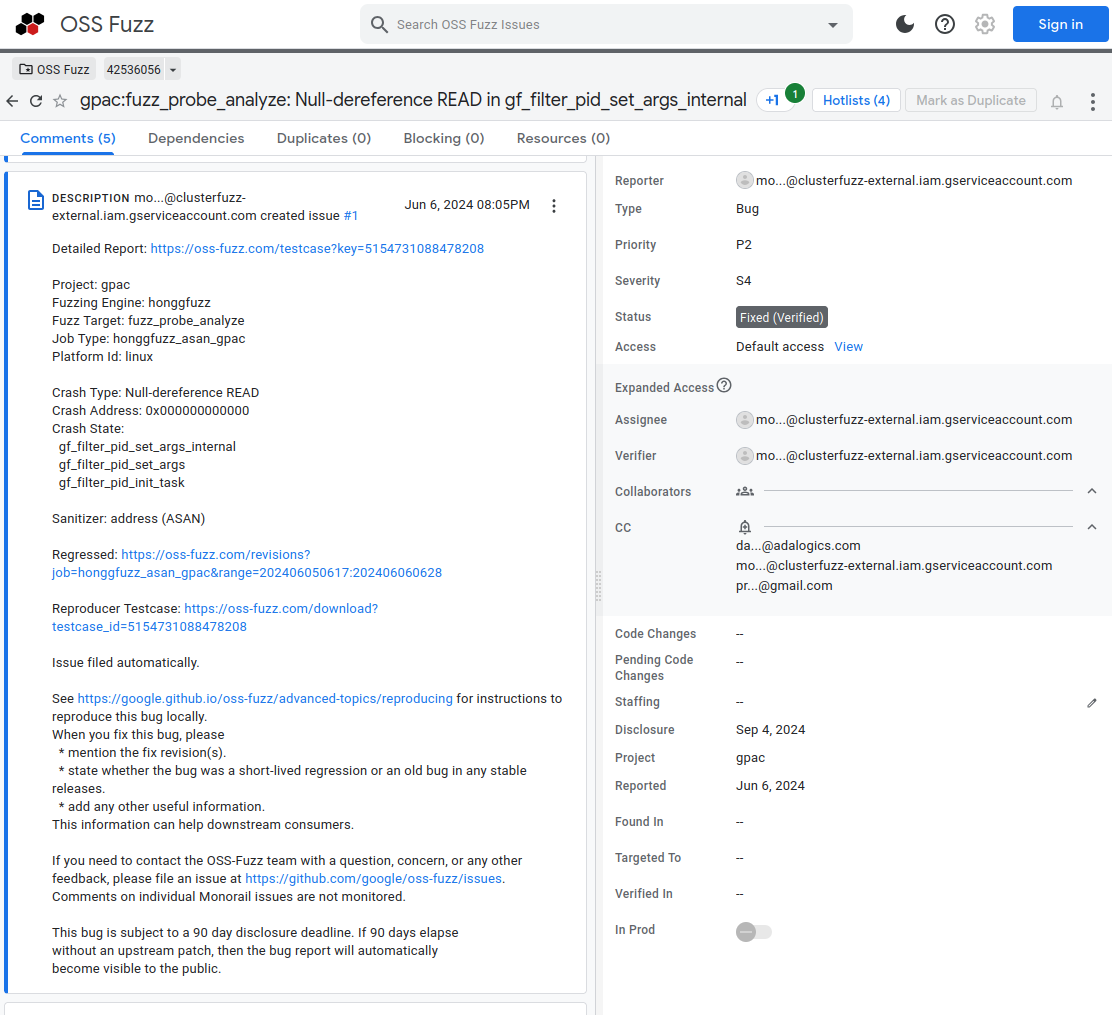
\includegraphics[width=0.69\paperwidth]{foto/issue.png}}
\caption{Example of bug report \cite{ossfuzz_bugtracker}}
\label{fig:issue}
\end{figure}
\ \\
At the moment of writing, the issue tracker platform was changed from "Monorail" to "Google Sites", so most of the work described here may no longer work as intended.




\newpage
Given that Monorail APIs could only be used by projects' developers registered to OSS-Fuzz and that there weren't any files that could be used for an offline analysis, I had to perform website scraping on the individual issues to retrieve the information. 
\newline
To do this, I used as reference a GitHub repository written by Zhen Yu Ding called "Monorail Scraper" \cite{scraper}, a tool to scrape and retrieve data from Monorail, that also included functionalities for ClusterFuzz-generated OSS-Fuzz issues.
\newline \newline
The tool relies on the Google Chrome web browser and their testing development tool called "ChromeDriver" \cite{driver}: this is an autonomous web server implementing "W3C WebDriver" \cite{driver_standard}, a standard providing a remote interface to control user-agents and a set of interfaces to perform analysis and manipulation of DOM elements.
\newline
Essentially, this allows the user to write scripts that, in turn, instruct the Google Chrome browser to visit a specific web page and possibly performs some interaction with it, like pushing a button, compiling a form or visiting another webpage by exploring the DOM elements.  
\newline \newline
In this work, I focused on the functionalities for the analysis of OSS-Fuzz reports.
\newline
Initially, the user provides a range of "report IDs" to retrieve.
\newline
Then, the tool opens a new Google Chrome instance and performs a connection to a specific link in the Monorail website, attempting the reconnection only once if the first one fails. If the resulting DOM shows a login form, it means that the requested bug is still in the disclosure window, in which case the next ID is analyzed.
\newline
Assuming that the requested report is publicly accessible, the DOM is scanned for key information.
During this phase, given that the project is already few years old, I had to make some minor corrections and adjustments as some parameters collected were changed and/or missing altogether.
\newline
All the information collected by each report was then stored in JSON files.
\newline
\begin{figure}[h]
\makebox[\textwidth][c]{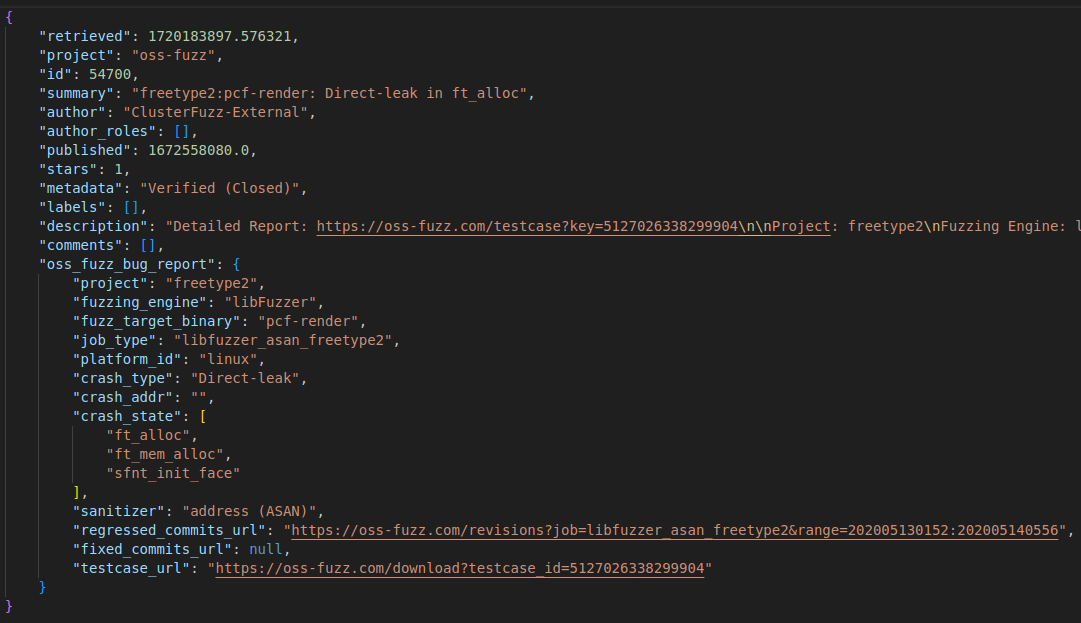
\includegraphics[width=0.66\paperwidth]{foto/json.png}}
\caption{Example of information collected from reports in JSON}
\label{fig:report}
\end{figure}
\ \\
The analysis was performed on all bugs between 2023-01-01 and 2024-06-31, for a total of 11743 collected reports.



\newpage
The second to last step was to analyze the previously obtained JSON files and make a list of the most bugged projects for each category.
\newline
To do this, I initially wrote a simple Python script that takes as input the JSON files and analyzes the information fields collected.
\newline
First, I checked the \textit{"metadata"} field for values like "WontFix", "Duplicate" or "Invalid": the first means that the developers themselves tagged that specific bug as non-relevant and will not be addressed in the future, the second refers to a report for a bug that has been already issued but triggered by a different testcase, while the last one means that the reported bug could not be reliably reproduced.
\newline
Then, I checked the \textit{"description"} field for manual reports, as they were not meaningful towards the final results. 
\newline
Assuming the report analyzed is valid and generated by ClusterFuzz, I retrieved the project name from the \textit{"oss\_fuzz\_bug\_report"} fields and used a dictionary key-value to keep track of the number of bugs reported for each project. 
\newline
\begin{figure}[h]
\centering
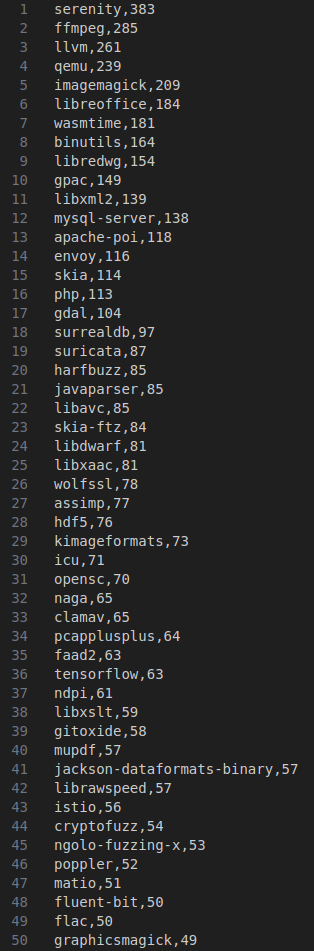
\includegraphics[scale=0.44]{foto/list.png}
\caption{Extract of the 50 most bugged projects}
\label{fig:list}
\end{figure}

\newpage
The last step was to analyze each project individually and determine which harness produced the highest number of reports.
\newline
Given the previous script, I extended it to take as input also a project name, so that the parsing of the JSON file focused only on reports for that particular project, and the dictionary key-value was now used to keep track of the number of bugs produced by each fuzzing target binary.
\ \\ \newline \newline
All this resulted in the following projects and harnesses being tested:
\begin{itemize}
  \item \textbf{All Sanitizers}
  \begin{itemize}
    \item binutils (fuzz\_objdump\_safe)
    \item harfbuzz (hb-subset-fuzzer)
    \item imagemagick (encoder\_heic\_fuzzer)
    \item libxml2 (valid)
    \item skia (skruntimeeffect)
  \end{itemize}
  \item \textbf{ASan + MSan}
  \begin{itemize}
    \item ghostscript (gs\_device\_pdfwrite\_fuzzer)
    \item libyang (lyd\_parse\_mem\_json)
    \item wasmedge (wasmedge-fuzztool)
    \item openjpeg (opj\_decompress\_fuzz\_J2K)
    \item myanmar-tools (zawgyi\_detector\_fuzz\_target)
  \end{itemize}
  \item \textbf{ASan + UBSan}
  \begin{itemize}
    \item cairo (svg-render-fuzzer)
    \item clamav (clamav\_dbload\_YARA\_fuzzer)
    \item freerdp (TestFuzzCoreClient)
    \item tarantool (luaL\_loadbuffer\_fuzzer)
    \item vlc (vlc-demux-dec-libfuzzer)
  \end{itemize}
  \item \textbf{ASan only}
  \begin{itemize}
    \item fwupd (uswid\_fuzzer)
    \item glslang (compile\_fuzzer)
    \item inchi (inchi\_input\_fuzzer)
    \item radare2 (ia\_fuzz)
    \item zeek (zeek-ftp-fuzzer)
  \end{itemize}
  \item \textbf{No Sanitizers}
  \begin{itemize}
    \item fluent-bit (flb-it-fuzz-cmetric\_decode\_fuzz\_OSSFUZZ)
    \item gpac (fuzz\_probe\_analyze)
    \item libdwarf (fuzz\_debug\_str)
    \item libredwg (llvmfuzz)
    \item serenity (FuzzJs)
  \end{itemize}
\end{itemize}








\newpage
\subsection{Testing with OSS-Fuzz}
The OSS-Fuzz repository contains several tools to build and test the available projects, as well as debugging and reproduction scripts.
\newline
Most of the tools used in this work are provided by the "helper.py" script, which I used to download a project's Docker image, build the fuzzers as well and download the public corpora made available by the developers.
\newline \newline
The commands used are:
\begin{verbatim}
    $ python3 helper.py pull_images 

    $ python3 helper.py build_image {project_name}

    $ python3 helper.py build_fuzzers {project_name}
        --sanitizer={address(default),memory,undefined,none} 
            --engine={libfuzzer(default),afl, honggfuzz, centipede}
        
    $ python3 helper.py download_corpora 
        --project={project_name} --fuzz-target={harness_name}
\end{verbatim}
\ \\
The \verb|pull_images| argument connects to OSS-Fuzz's Google Bucket to download and update all the Docker "base images" on your local machine, which are used by all projects as the base image to create their respective testing environment.
\newline \newline
The \verb|build_image| argument takes as input the name of a project and builds its Dockerfile, creating a new image on your local machine that will be later used to perform fuzzing. During this process, all dependencies and resources needed to correctly compile the fuzzers are downloaded and installed, including the main \textit{build.sh} script. It was used in conjunction with daily \verb|git pull| on the OSS-Fuzz repository, to make sure that I was always building the latest version. 
\newline \newline
The \verb|build_fuzzers| argument takes as input the name of a project and a list of possible sanitizers and fuzzing engines to be used during the compilation of the fuzz targets. Although this command accepts only one sanitizer and fuzzing engine at a time, it's possible to mix them by acting on some environment variables provided by the base images. Finally, this script acts as a "wrapper" for a much more complex Docker command, that creates the project's Docker image using some specific environment variables and invokes the execution of the \textit{build.sh} script.
\newline \newline
The \verb|download_corpora| argument takes as input a project name and a fuzz target, it then connects to the project's Google Bucket and downloads the latest public corpus for the provided fuzz target.
\newline \newline \newline
After executing these commands, three new directories are created.
\newline
The "out" directory contains the project's directory where all the built files are saved, including libraries, fuzz targets and other files created by the selected fuzzer.
\newline
The "work" directory acts as a temporary location to store intermediate files during the building process, it may also we used to store the fuzzing session results.
\newline
The "corpus" directory contains the downloaded corpora stored as zip files.



\newpage
To prepare the tests, I was tasked with building the chosen harnesses using all possible values for sanitizers, meaning that each project was compiled 4 times: with ASan only, with MSan only, with UBSan only and without any sanitizer.
\newline
Moreover, all projects were built using AFL as fuzzing engine, because (perché abbiamo usato AFL ???) 
\newline \newline
The tests were performed inside each project's Docker image, created and configured using the following command:
\begin{verbatim}
    $ docker run --rm --privileged --platform linux/amd64 
        -v /oss-fuzz/build/out/{project_name}/:/out/
        -v /oss-fuzz/build/corpus/{project_name}/:/corpus/    
        -v /home/zio-saba/Scrivania/TESI/logfiles/:/logfiles/ 
        -it  gcr.io/oss-fuzz/{project_name} /bin/bash
\end{verbatim}
\ \\
This is a shorter and modified version of the command invoked by the \verb|build_fuzzer| wrapper.
\newline \newline
The first few parameters are needed to create a privileged instance of Docker and specify the running platform on which the fuzz targets will be tested.
\newline \newline
The arguments starting with \verb|-v| are used to create a shared directory in the Docker container, which means linking a local directory to a virtual one created inside the container. This was needed to make sure that I could access the resources stored locally on my machine (i.e. fuzz targets, libraries and their corpus) from inside the Docker container used for the tests.
\newline \newline
The last line invokes the project image to load as well as making it interactive by spawning a \verb|/bin/bash| process.
\newline \newline \newline \newline
Once the Docker images has been loaded and ready to use, some final adjustments were performed to perform the tests.
\newline \newline
All tests performed on fuzz targets built with MSan required the sanitizer's libraries to be copied in some specific locations, using the following commands:
\begin{verbatim}
    $ cp -R /usr/msan/lib/* /usr/local/lib/x86_64-unknown-linux-gnu/
    $ cp -R /usr/msan/include/* /usr/local/include
\end{verbatim}
\ \\
All tests performed on fuzz targets built without sanitizers relied on Valgrind to perform binary analysis and profiling, installed using the following command:\begin{verbatim}
    $ sudo apt install gdb valgrind
\end{verbatim}
\ \\
Sometimes, the "APT" tool was not available in a specific Docker container: this is because all base images provided by OSS-Fuzz contain a minimal installation of Linux Ubuntu with only some key packages that are usually enough to compile a programs, such as compiler, assembler, text editors and standard libraries.
\newline
In such cases, the \verb|unminimize| command was executed, which essentially "unpacks" the container and reverts it to a standard Ubuntu image, reinstalling all the default packages as well as standard additional tools.



\newpage
When testing fuzz targets built with ASan, MSan or UBSan, I used the following command:
\begin{verbatim}
    $ for i in /corpus/*; do 
        echo "TEST" $i; 
        echo "TEST" $i >> /logfiles/PROJECT_SANITIZER-NAME.log; 
        ./{fuzz_target} $i &>> /logfiles/PROJECT_SANITIZER-NAME.log; 
      done
\end{verbatim}
\ \\
This commands uses the shell \verb|for| construct to scan all files found in the "corpus" directory.
\newline
Then, it prints the name of the current testcase on the terminal, which I used for monitoring purposes.
\newline
Finally, it prints the name of the current testcase on a log file followed by the results of the fuzz target executed on that particular testcase.
\newline
\begin{figure}[h]
\makebox[\textwidth][c]{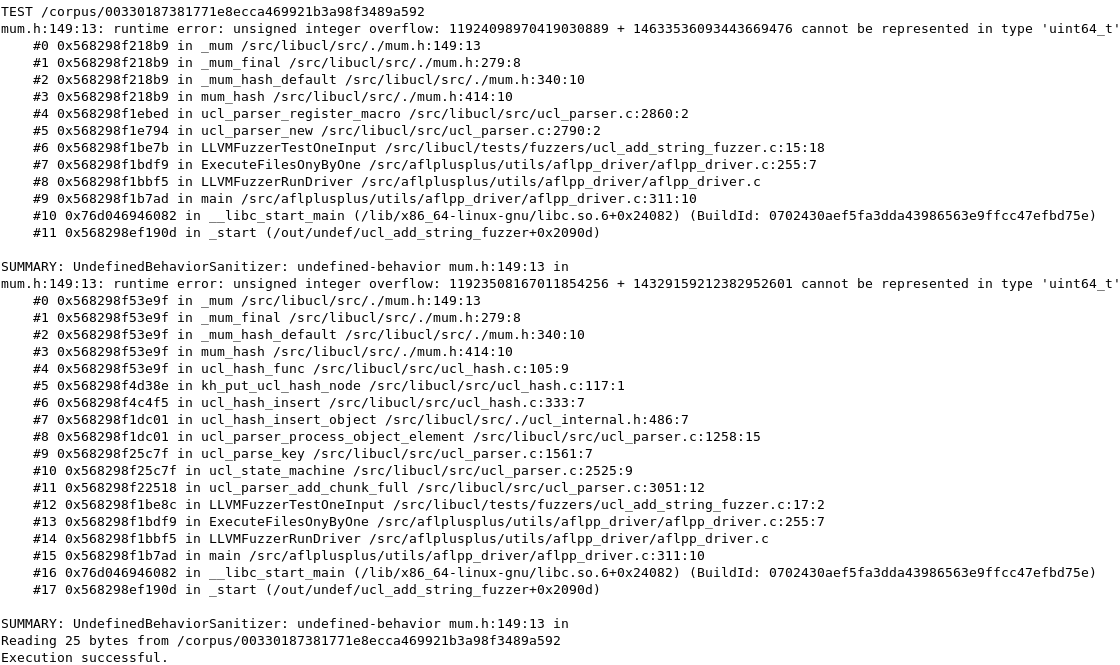
\includegraphics[width=0.8\paperwidth]{foto/ubsan_example.png}}
\caption{Example of integer-overflow bug reported by UBSan}
\label{fig:ubsan_example}
\end{figure}
\ \\



\newpage
When testing fuzz targets built without any sanitizers, I used Valgrind to analyze and profile the binary execution, useing the following command:
\begin{verbatim}
    $ for i in /corpus/*; do 
        echo "TEST" $i; 
        valgrind --log-fd=9 9>>/logfiles/PROJECT_valgrind.log 
            ./{fuzz_target} $i >> /logfiles/PROJECT_valgrind.log 
            && echo -e "\n\n" >> /logfiles/PROJECT_valgrind.log; 
      done
\end{verbatim}
\ \\
Again, I used the shell \verb|for| construct to scan all files found in the "corpus" directory and print the name of the current testcase on the terminal for monitoring purposes.
\newline
Then, I invoked Valgrind with a custom file descriptor, which allowed me to capture \verb|STDERR| and print it in the log file.
\newline
Finally, it prints the result of the fuzz target executed on that particular testcase and adds some newline characters to make the log file more readable.\newline
\begin{figure}[h]
\makebox[\textwidth][c]{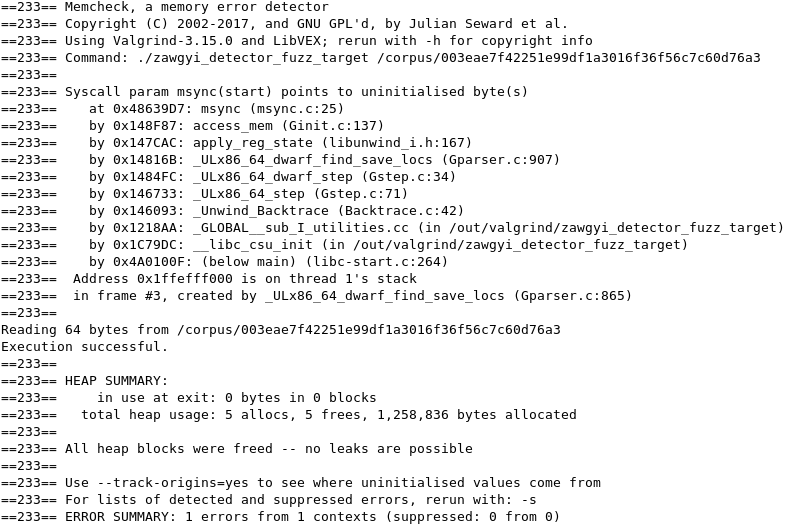
\includegraphics[width=0.65\paperwidth]{foto/valgrind_example.png}}
\caption{Example of use-of-uninitialised-memory (UUM) bug reported by Valgrind}
\label{fig:valgrind_example}
\end{figure}
\ \\




\newpage
Finally, not all projects built on their first attempt.
\newline \newline
In most cases, the building process failed due to missing libraries: for example, libraries like \verb|pthread| and \verb|math| were often automatically added by the sanitizers.
\newline
Other times, libraries were not being correctly linked and/or were missing crucial compiling flags, like \verb|-ldl| and \verb|-lz|.
\newline \newline
To fix these problems, I had to manually modify the source files and compile the fuzz targets from inside the Docker container, using a command similar to the one executed by \verb|compile_fuzzers|:
\begin{verbatim}
    $ docker run --rm --privileged --platform linux/amd64 
        -e PROJECT_NAME={project_name} -e HELPER=True 
        -e FUZZING_LANGUAGE=c++ 
        -e FUZZING_ENGINE=afl 
        -e SANITIZER={address,memory,undefined,none} 
        -v /oss-fuzz/build/out/{project_name}/:/out/
        -v /oss-fuzz/build/corpus/{project_name}/:/corpus/    
        -v /oss-fuzz/build/work/{project_name}/:/work/
        -it  gcr.io/oss-fuzz/{project_name} /bin/bash
\end{verbatim}
\ \\
Similarly to before, the first few parameters are needed to create a privileged instance of Docker and specify the running platform on which the fuzz targets will be tested, the arguments starting with \verb|-v| are used to create a shared directory in the Docker container and the last line invokes the project image to load as well as making it interactive by spawning a \verb|/bin/bash| process.
\newline \newline
The novelty lies in the arguments starting with \verb|-e|, which can be used to override the environment variables provided by the Docker image.
\newline
These variables can be used by the source files to compile a program using the most appropriate compile flags, fuzzing engine and sanitizers, and they can be easily modified by the user when creating the Docker image to easily re-target the compilation with little to none effort.
\newline \newline
After loading the Docker image and modifying the source files, the command \verb|compile| invokes the execution of the "build.sh" script and starts the building process for the fuzz targets.




\newpage
\subsubsection{??? Un singolo esempio di test mostrato per intero ???}

\newpage
\section{FuzzBench}
\subsection{Selecting the projects}
Explain the selection process and the chosen test set...
\newline \newline
Explain how the experiment\_project.yaml analysis was performed...
\newline \newline
Explain how crashes and corpus were obtained through scraping...
\newline \newline
\subsection{Testing with FuzzBench}
Explain how projects were built....
\newline \newline
Explain how tests were automated and their duration...
\subsubsection{??? Un singolo esempio di test mostrato per intero ???}


\newpage
When i testef fuzzbench and had to build using ASan + UBSan, i Didi this:
\begin{verbatim}
    $ docker run --rm --privileged --platform linux/amd64 
        -e PROJECT_NAME={project_name} -e HELPER=True 
        -e FUZZING_LANGUAGE=c++ -e FUZZING_ENGINE=afl 
        -e SANITIZER=address 
        -e SANITIZER_FLAGS_address="
            -fsanitize=address,array-bounds,bool,builtin,enum,
                integer-divide-by-zero,null,object-size,return,
                returns-nonnull-attribute,shift,
                signed-integer-overflow,unsigned-integer-overflow,
                unreachable,vla-bound,vptr
            -fno-sanitize-recover=array-bounds,bool,builtin,enum,
                integer-divide-by-zero,null,object-size,return,
                returns-nonnull-attribute,shift,
                signed-integer-overflow,unreachable,
                vla-bound,vptr 
            -fsanitize-address-use-after-scope" 
        -v /oss-fuzz/build/out/{project_name}/:/out/  
        -v /oss-fuzz/build/work/{project_name}/:/work/
        -it  gcr.io/oss-fuzz/{project_name} /bin/bash
\end{verbatim}

